\subsection{Propósito y alcance}
El archivo \texttt{SDCMotor.cpp} implementa una \emph{S-Function Level-2} para Simulink cuyo objetivo es actuar como puente entre el modelo de control y un módulo de E/S analógicas OPTO22 (vía Ethernet), utilizando la librería \texttt{O22SIOMM} (clase \texttt{O22SnapIoMemMap}). En cada paso de simulación el bloque:
\begin{itemize}
    \item \textbf{envía} al OPTO22 dos comandos analógicos: comando de voltaje para el actuador, y  una corriente de carga (\texttt{iLoad})\footnote{El significado físico exacto depende de la conexión real.};
    \item \textbf{recibe} desde el OPTO22 dos mediciones analógicas:  velocidad (\texttt{velocidad}) y  corriente (\texttt{corriente});
    \item \textbf{detiene} la simulación si se acumulan demasiados errores de comunicación.
\end{itemize}



\subsubsection{Red y configuración fija en el código}
La S-Function abre la comunicación Ethernet con un \emph{Brain} OPTO22 en la IP \texttt{192.168.6.101} y puerto \texttt{2001}. Por lo tanto, el PC y el equipo OPTO22 deben estar en la misma red/subred y sin bloqueo por firewall/ACL. (Estos valores están embebidos en \texttt{SDCMotor.cpp}; si se cambia el setup, deben actualizarse en el código o parametrizarse.)

\subsubsection{Requisitos de compilación (MEX/S-Function)}
Para generar el binario \texttt{SDCMotor.mex*} se requiere:
\begin{itemize}
    \item \textbf{Un compilador C/C++ soportado por MATLAB} configurado con \texttt{mex -setup C++}.
    \item \textbf{Headers y librería} de OPTO22 (\texttt{O22SIOMM.h} y la correspondiente \texttt{.lib/.dll} o fuentes) disponibles en rutas conocidas.
\end{itemize}
MATLAB permite especificar rutas de \emph{include} con \texttt{-I} y enlazado con opciones de librería durante \texttt{mex}.

\subsubsection{Compilación recomendada desde MATLAB}
Desde la carpeta donde reside \texttt{SDCMotor.cpp}, compilar preferentemente con:
\begin{verbatim}
mex -v SDCMotor.cpp ...
    -I"<RUTA_OPTO22>\include" ...
    -L"<RUTA_OPTO22>\lib" -lO22SIOMM
\end{verbatim}

\noindent Si la distribución de OPTO22 entrega la implementación como fuentes (por ejemplo, \texttt{O22SIOMM.cpp}), una alternativa directa es:
\begin{verbatim}
mex -v SDCMotor.cpp O22SIOMM.cpp -I"<RUTA_OPTO22>\include"
\end{verbatim}

\noindent Tras compilar, el archivo \texttt{SDCMotor.mex*} debe quedar en el \emph{MATLAB path} o en el mismo directorio del modelo para que Simulink pueda cargar el bloque.

\subsection{Dependencias y compilación}
\begin{itemize}
    \item \textbf{API Simulink:} \texttt{simstruc.h} para la definición de S-Functions.
    \item \textbf{OPTO22:} \texttt{O22SIOMM.h} y la implementación asociada de la librería (debe estar disponible al compilar el MEX).
\end{itemize}

\noindent La S-Function se declara como:
\begin{verbatim}
#define S_FUNCTION_NAME  SDCMotor
#define S_FUNCTION_LEVEL 2
\end{verbatim}
y se encapsula en \texttt{extern C} para asegurar \emph{linkage} compatible con el mecanismo de carga de Simulink.

\subsection{Parámetros del bloque}
El bloque define \textbf{un (1) parámetro} de máscara:
\begin{itemize}
    \item \textbf{P1:} tiempo de muestreo $T_s$ (segundos). Se lee en \texttt{mdlInitializeSampleTimes()} mediante:
    \[
        T_s \leftarrow \texttt{mxGetScalar(ssGetSFcnParam(S,0))}
    \]
\end{itemize}
Si la cantidad de parámetros provistos en Simulink no coincide con lo esperado, \texttt{mdlInitializeSizes()} retorna y Simulink reporta el error.

\subsection{Interfaz de entradas y salidas}
El bloque tiene \textbf{2 entradas escalares} y \textbf{2 salidas escalares}, todas tipo \texttt{real\_T}:

\begin{table}[h]
\centering
\begin{tabular}{lll}
\hline
\textbf{Puerto} & \textbf{Señal} & \textbf{Descripción} \\
\hline
Entrada 0 & $u$      & Comando de voltaje a enviar al OPTO22 (canal analógico 0). \\
Entrada 1 & $iLoad$  & Corriente de carga a enviar al OPTO22 (canal analógico 1). \\
\hline
Salida 0 & $y$      & Velocidad leída desde OPTO22 (canal analógico 4). \\
Salida 1 & $z$      & Corriente leída desde OPTO22 (canal analógico 6). \\
\hline
\end{tabular}
\caption{Mapa de puertos de Simulink a puntos analógicos OPTO22.}
\label{tab:sdcmotor_ports}
\end{table}

\noindent Además, se exige memoria contigua para ambas entradas (\texttt{ssSetInputPortRequiredContiguous}), lo que simplifica el acceso a las señales.

\subsection{Vectores de trabajo y estados}
Para mantener información entre llamados, la S-Function reserva:
\begin{itemize}
    \item \textbf{PWork (1 puntero):} almacena un puntero a la instancia \texttt{O22SnapIoMemMap} que representa la conexión activa con el OPTO22.
    \item \textbf{IWork (1 entero):} contador de errores de comunicación (\texttt{WORK\_INT\_ERROR\_COUNT}).
\end{itemize}
Se define además \textbf{1 estado discreto} (\texttt{ssSetNumDiscStates(S,1)}), aunque en esta implementación no se observa uso explícito de \texttt{ssGetX}/\texttt{ssSetX}; en la práctica, la memoria persistente relevante queda cubierta por \texttt{PWork} e \texttt{IWork}.

\subsection{Manejo de errores}
El bloque implementa un mecanismo simple de tolerancia a fallos:
\begin{itemize}
    \item Cada vez que una operación de lectura/escritura hacia OPTO22 retorna un código distinto de \texttt{SIOMM\_OK}, se incrementa \texttt{IWork[ERROR\_COUNT]} y se imprime un mensaje vía \texttt{ssPrintf}.
    \item Si el contador supera \texttt{MAX\_ERROR\_COUNT} (definido como 5), se invoca \texttt{ssSetErrorStatus(S, "...")} y Simulink detiene la ejecución del modelo.
\end{itemize}

\subsection{Ciclo de vida del bloque (funciones S-Function)}
A continuación se describe el rol de cada función obligatoria/registrada y el flujo típico en simulación.

\subsubsection{\texttt{mdlInitializeSizes(S)}: declaración de capacidades}
Configura la firma del bloque: número de parámetros, puertos de entrada/salida, tiempos de muestreo y tamaños de vectores de trabajo. En particular:
\begin{itemize}
    \item 1 parámetro esperado.
    \item 2 entradas escalares y 2 salidas escalares.
    \item 1 tiempo de muestreo.
    \item \texttt{PWork} para el objeto de interfaz OPTO22 y \texttt{IWork} para el contador de errores.
\end{itemize}

\subsubsection{\texttt{mdlInitializeSampleTimes(S)}: tiempo de muestreo}
Asigna el tiempo de muestreo del bloque a partir del parámetro $T_s$ y fija offset en 0:
\[
    T_s = \texttt{Param(0)}, \qquad \text{offset} = 0.
\]

\subsubsection{\texttt{mdlStart(S)}: apertura de conexión con OPTO22}
Se ejecuta una sola vez al inicio. Sus pasos son:
\begin{enumerate}
    \item Crea el objeto \texttt{Brain = new O22SnapIoMemMap()}.
    \item Abre conexión Ethernet con:
    \begin{itemize}
        \item IP: \texttt{192.168.6.101}
        \item Puerto: \texttt{2001}
        \item Timeout: \texttt{10000} (ms)
        \item Último argumento: \texttt{1} (dependiente de la API; típicamente flags/modo).
    \end{itemize}
    \item Espera a que la apertura finalice consultando \texttt{IsOpenDone()} mientras retorne 
    
    \texttt{SIOMM\_ERROR\_NOT\_CONNECTED\_YET}.
    \item Si ocurre un error, define un estado de error fatal:
    \begin{center}
        \texttt{"Unable to connect to OPTO22 (192.168.6.101)."}
    \end{center}
    \item Si la conexión es exitosa, guarda el puntero del objeto en \texttt{ssGetPWork(S)[0]} e inicializa el contador de errores en 0.
\end{enumerate}

\subsubsection{\texttt{mdlUpdate(S,tid)}: escritura de comandos (salida hacia planta)}
En cada paso de simulación, el bloque toma las entradas de Simulink y las envía al OPTO22:
\begin{itemize}
    \item Entrada 0 ($u$) $\rightarrow$ \texttt{SetAnaPtValue(0, (float)*u)}.
    \item Entrada 1 ($iLoad$) $\rightarrow$ \texttt{SetAnaPtValue(1, (float)*iLoad)}.
\end{itemize}
Cada envío es verificado; ante error se incrementa el contador y, si se supera el umbral, se detiene la simulación.

\paragraph{Nota.}
El mensaje impreso ante error en el segundo envío repite el texto \texttt{Error sending voltage command.\textbackslash n}; si se quiere mayor trazabilidad, se puede diferenciar mensajes (p.ej. ``voltage'' vs ``load current'').

\subsubsection{\texttt{mdlOutputs(S,tid)}: lectura de mediciones (entrada desde planta)}
En cada paso, el bloque consulta dos valores analógicos:
\begin{itemize}
    \item Velocidad: \texttt{GetAnaPtValue(4, \&velocidad)} $\rightarrow y = \texttt{(real\_T)velocidad}$.
    \item Corriente: \texttt{GetAnaPtValue(6, \&corriente)} $\rightarrow z = \texttt{(real\_T)corriente}$.
\end{itemize}
Las lecturas tienen la misma política de manejo de errores descrita previamente.

\subsubsection{\texttt{mdlTerminate(S)}: cierre seguro}
Al terminar la simulación:
\begin{enumerate}
    \item Recupera el objeto desde \texttt{PWork}.
    \item Envía \textbf{0.0} al canal analógico 0 (\texttt{SetAnaPtValue(0,0.0)}) como acción de seguridad para dejar el comando de voltaje en cero.
    \item \hl{\textbf{AGREGAR: Brain->SetAnaPtValue(1,0.0); para cierre seguro del nuevo canal!!!!!!!}}
    \item Cierra la conexión (\texttt{Close()}).
    \item Libera memoria (\texttt{delete Brain}).
\end{enumerate}

\subsection{Resumen operacional (pseudoflujo)}
\begin{verbatim}
Start:
  conectar a OPTO22 (IP fija)
  error_count = 0

Cada Ts:
  mdlUpdate:
    enviar u -> AO0
    enviar iLoad -> AO1
  mdlOutputs:
    leer velocidad <- AI4
    leer corriente <- AI6
  si error_count > 5:
    detener simulación

Terminate:
  AO0 = 0
  AO1 = 0
  cerrar conexión
\end{verbatim}

\begin{figure}
    \centering
    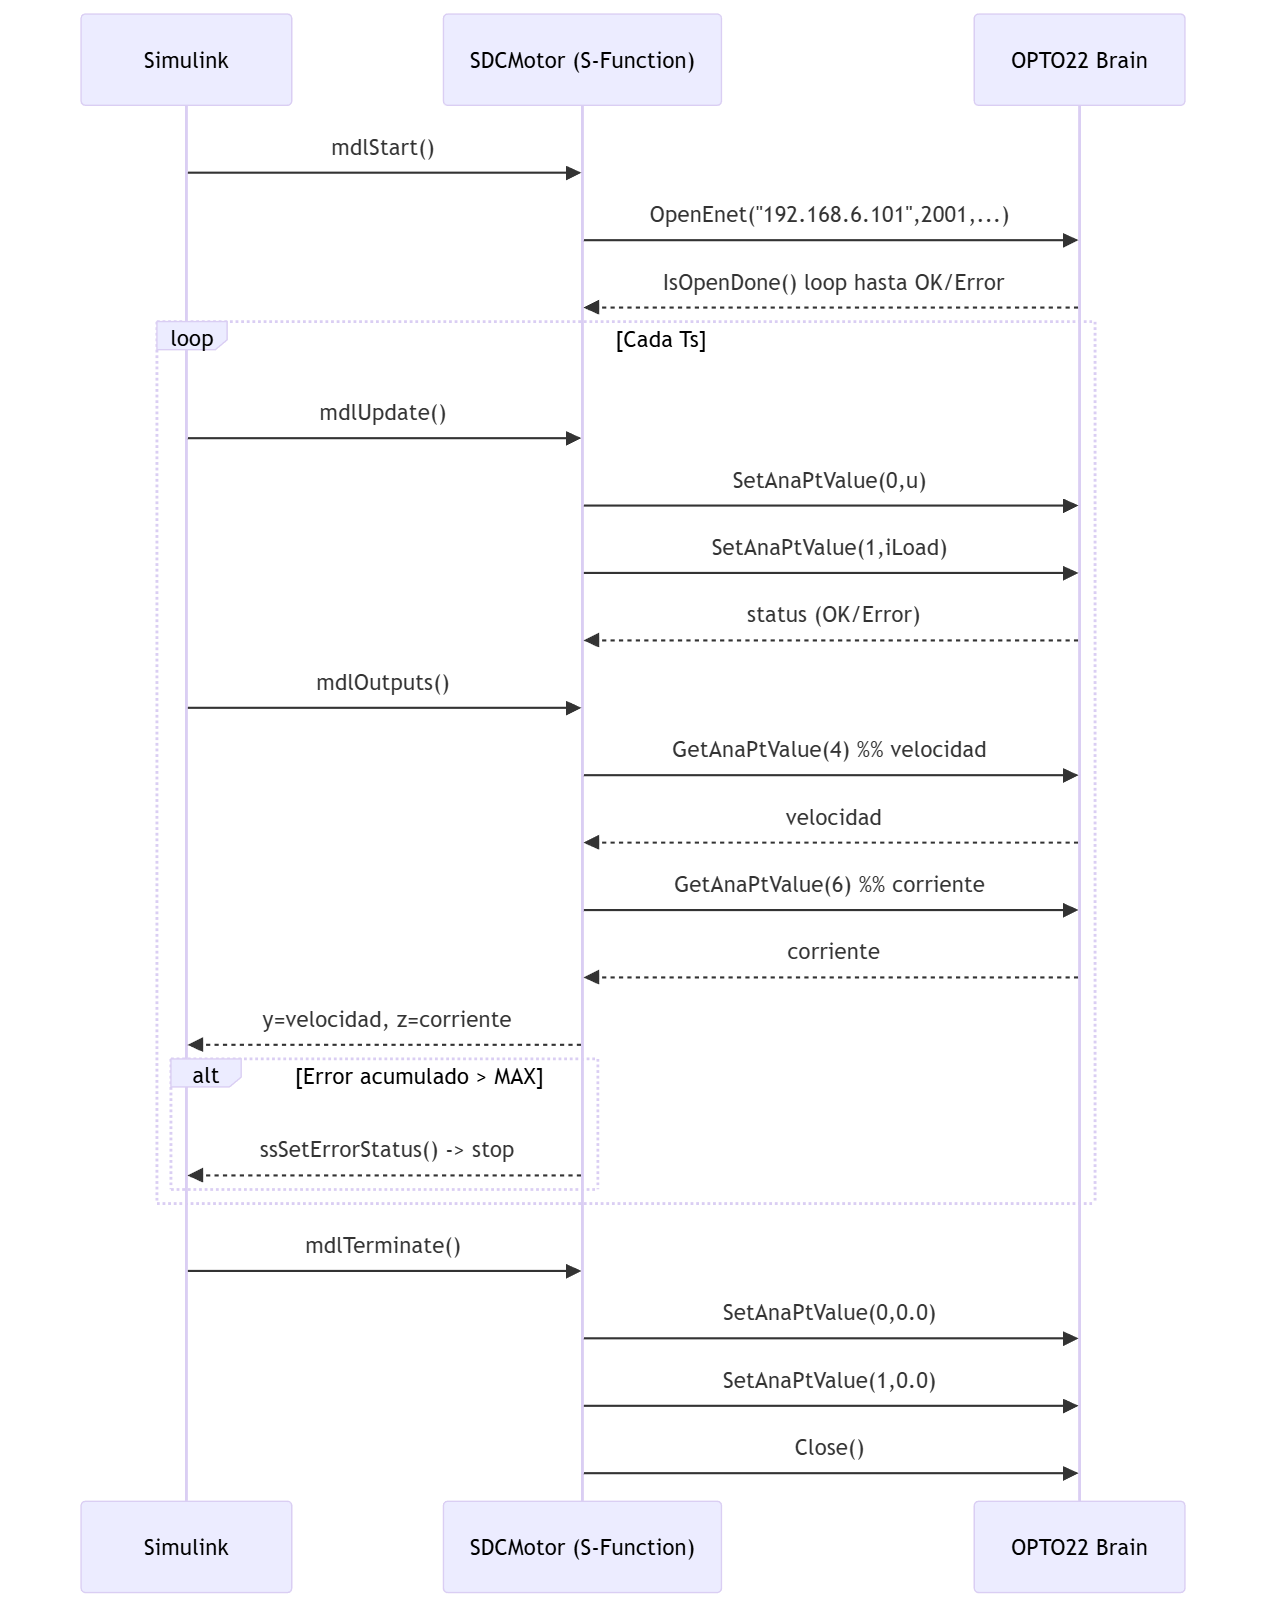
\includegraphics[width=0.7\textwidth]{img/SDCMotor/SDCMotor_diagram.png}
    \caption{Caption}
    \label{fig:SDCMotor diagram}
\end{figure}

\subsection{Consideraciones de integración y configuración}
\begin{itemize}
    \item \hl{\textbf{IP de computador HOST:} \textbf{PONER ESAS COSAS DE LA IP DEL PC ESPECIAL}}
    \item \textbf{IP fija en el código:} la dirección \texttt{192.168.6.101} está embebida. Para reutilización en distintas configuraciones de red, es recomendable parametrizar IP/puerto como parámetros del bloque.
    \item \textbf{Entradas Analógicas adicionales:} En la configuración actual del setup, solo se ocupan 2 de los 4 puntos de entrada del modulo  \texttt{SNAP-AIV-4} \cite{opto22_snap_aiv4}, pero habilitar puntos adicionales puede incrementar el overhead y prohibir el uso de tiempos de muestreo menores.
    \item \textbf{Mapa de canales:} los índices (0,1,4,6) asumen una asignación concreta de puntos analógicos en el OPTO22. Cualquier cambio de cableado/escala debe reflejarse en este mapa o, idealmente, parametrizarse.
    \item \textbf{Escalamiento físico:} este bloque transmite y recibe valores \texttt{float} sin aplicar conversión (p.ej., V$\leftrightarrow$RPM). Si se requiere trazabilidad metrológica, conviene documentar (y/o implementar) funciones de escala y saturación directamente en la simulación.
    \item \textbf{Robustez:} el umbral de errores (\texttt{MAX\_ERROR\_COUNT=5}) detiene la simulación. Esto es útil como medida de seguridad.
\end{itemize}